\label{texfile:SWF}
The \swf\ domain is a 2D network of cells which is usually, but not necessarily, coincident with the top of the \gwf\ domain.

\mfus\ allows individual (i.e.\ \gwf, \swf\ and \cln)  processes  to add to the global
conductance matrix in order to represent fluxes between cells
within a process as well as with cells of other processes.
\mfus\ provides a framework for tightly
coupling multiple hydrologic processes. The tight coupling, in
contrast to a sequential or iterative coupling approach, occurs
through the formulation of a global conductance matrix that
includes the cells for all processes.

The flows between \swf\ cells are governed by the diffusion-wave equations, which ultimately provide a pressure head (i.e. surface water depth) at each cell.

\subsection{Generating a \swf\ Domain}
A \swf\ domain can be easily added to the \mfus\ model using the same template mesh that was used to define the \gwf\ mesh, as described in Section~\ref{texfile:TemplateMesh}.

The \swf\ domain is generated using this instruction:

\ins{generate swf domain}
    {This subtask currently has only one instruction that is used to define:
     \begin{itemize}
        \item Top elevation (i.e. $z$-coordinate, ground surface elevation)
    \end{itemize}

    It reads instructions until an \textsf{end} instruction is found e.g.\:


    {\Large \sf end generate swf domain}
    }

Here, the \textsf{top elevation} instruction has the same options as described in Section~\ref{section:topelev} for the \gwf\ domain.

Currently, the element zone numbering for the \swf\ domain is determined by the instruction used to generate the template mesh:
\begin{description}
  \item[2d mesh from gb] The \gb\ element area numbers are used to define the \mfus\ element zone numbers.
  \item[generate uniform rectangles] The element zone numbers default to 1.
\end{description}

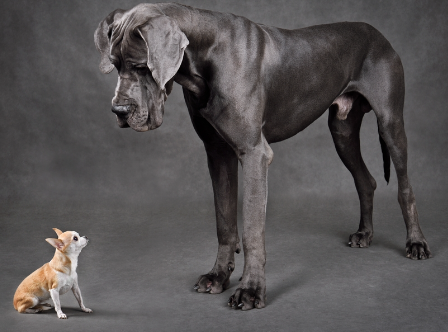
\includegraphics[width=.15\textwidth]{ModelDevelopment} \textit{We should provide instructions for defining swf zone numbers, e.g.\ from a cell list or raster file.}

\subsubsection{Cell Connection Properties}  \index{\swf\ Domain ! cell connection properties}
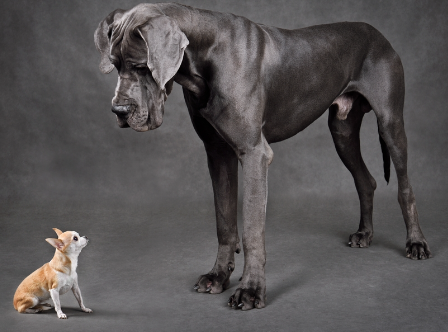
\includegraphics[width=.15\textwidth]{ModelDevelopment} \textit{
\swf\ cell to \swf\ cell connection properties are automatically defined by \mut\ based on control-volume approach and element type. The code needs to be checked, verified and documented more completely.}

These \swf\ cell connection properties vary on a cell-by-cell basis:
\begin{itemize}
     \item The \swf-\gwf\ connection length.
     \item The \swf-\gwf\ connection area.
\end{itemize}

Cell selections must first be made using the instructions described on page~\pageref{page:cellSelect} for the \gwf\ domain.

Currently, \mut\ assigns a default value of 0.001 $m$ for the \swf\ cell to \gwf\ cell connection length, and this instruction allows you to change it:

\ins{swf to gwf connection length}
    {
        \squish
        \begin{enumerate}
        \item \rnum{value}  \swf\ cell to \gwf\ cell connection length [$L$].
        \end{enumerate}
          A \swf\ cell to \gwf\ cell connection length \rnum{value} is assigned to the chosen cells.
    }

Currently, \mut\ assigns a \swf-\gwf\ connection area depending on which control volume approach is used :
\begin{description}
\item [Mesh-centred approach] The connection area will be calculated as the template mesh element area (i.e.\ the yellow triangle shown on page~\pageref{page:MeshCentredApproach}).
\item [Node-centred approach] The connection area will be calculated as  the contibuting area of neighbouring template mesh elements (i.e.\ the yellow polygon shown on page~\pageref{page:NodeCentredApproach}).
\end{description}

\subsubsection{Assigning Material Properties}  \index{\swf\ Domain ! material properties}
Unlike the \gwf\ domain, \swf\ domain material properties vary on a zone-by-zone basis, which means assigning material property values are done using zone selections instead of cell selections.

%\swf\ material properties that vary on a zone-by-zone basis are:
%\begin{itemize}
%     \item Manning's coefficient of friction.
%     \item Depression storage height.
%     \item Obstruction storage height.
%     \item \swf\ depth for smoothing (h1 and h2)
%\end{itemize}
%
Prior to making cell or zone selections and assigning properties, we need to activate the \swf\ domain using these instructions:
\begin{verbatim}
    active domain
    swf
\end{verbatim}

Zone selections must first be made using the instructions described on page~\pageref{page:zoneSelect} for the \gwf\ domain, then these instructions can be used to assign material properties to the current zone selection:

\ins{swf manning}
    {
        \squish
        \begin{enumerate}
        \item \rnum{value}  Manning's coefficient of friction [$L^{-1/3} T$].
        \end{enumerate}
          A Manning's coefficient of \rnum{value} is assigned to the chosen cells.
    }

\ins{swf depression storage height}
    {
        \squish
        \begin{enumerate}
        \item \rnum{value}  Depression storage height [$L$].
        \end{enumerate}
          A depression storage height of \rnum{value} is assigned to the chosen zones.
    }

\ins{swf obstruction storage height}
    {
        \squish
        \begin{enumerate}
        \item \rnum{value}  Obstruction storage height [$L$].
        \end{enumerate}
          An obstruction storage height of \rnum{value} is assigned to the chosen zones.
    }

\ins{swf depth for smoothing}
    {
        \squish
        \begin{enumerate}
        \item \rnum{value1}  Depth for smoothing height 1 [$L$].
        \item \rnum{value2}  Depth for smoothing height 2 [$L$].
        \end{enumerate}
          Two depth for smoothing heights are read in \rnum{value1} and \rnum{value2} and assigned to the chosen zones.
    }

A lookup table of \swf\ material properties  is provided in the file \texttt{qrySWFMaterials.txt}, located in the \bin\ directory as outlined on page~\pageref{page:userbin}.

In order for \mut\ to access the lookup table, you first need to provide a link to this file using the instruction:

\ins{swf materials database}
    {
        \squish
        \begin{enumerate}
        \item \str{file}  \swf\ material properties lookup table file name.
        \end{enumerate}
          \mut\ uses the file \str{file} to look up \swf\ material properties.
    }

You can now assign a full set of \swf\ material properties to the current zone selection, as described on page~\pageref{page:zoneSelect}, using this instruction:

\ins{chosen zones use swf material number}
    {
        \squish
        \begin{enumerate}
        \item \inum{val}  \swf\ material ID number.
        \end{enumerate}
          A unique set of \swf\ material properties is retrieved from a lookup table, using the given  material ID number \inum{val}, and assigned to the chosen zones.
    }

The assigned \swf\ material properties are written to the screen and \texttt{.eco} file:
\begin{verbatim}
    chosen zones use swf material number
    	Assigning all chosen SWF zones properties of material 1.0000, Streambed
    	Manning's Coefficient:          3.00000E-02
    	Depression Storage Height:      0.10000
    	Obstruction Storage Height:      0.0000
    	SWF Smoothing Depth 1:          1.00000E-06
    	SWF Smoothing Depth 2:          1.00000E-06
\end{verbatim}

You can find detailed information about how to use \dbase\ to modify or define your own lookup tables in Tutorial~\ref{tecfile:DbaseUseage}.

\subsubsection{Initial Conditions}  \index{\swf\ Domain ! initial condition ! initial (starting) depth}
An initial (or starting) head should be assigned to each cell in the \swf\ domain.  This could be an initial guess at the beginning of a transient stress period or a set of hydraulic heads from a previous run.

To assign an initial head to the \swf\ model domain, you must first make a cell selection as described on page~\pageref{page:cellSelect}, then this instruction can be used to calculate an initial (or starting) head for the flow solution given an initial surface water depth:

\ins{swf initial depth}
    {
        \squish
        \begin{enumerate}
        \item \rnum{value}  Initial depth [$L$].
        \end{enumerate}
          An initial depth of \rnum{value} is used to calculate an initial head at each of the chosen cells.
    }

\subsubsection{Boundary Conditions}  \index{\swf\ Domain ! boundary conditions}
A constant head boundary condition fixes the head at a \swf\ cell at a given value, allowing water to flow into or out of the \swf\ model domain depending on surrounding conditions.    To assign a uniform constant head to the \swf\ model domain use this instruction:

\ins{swf constant head}
    {
        \squish
        \begin{enumerate}
        \item \rnum{value}  Constant hydraulic head [L].
        \end{enumerate}
          An constant hydraulic head  of \rnum{value} is assigned to the chosen cells.
    }

A recharge boundary condition forces  water to flow in to the \swf\ model domain at a specified rate.   To add recharge  to the \swf\ model domain use this instruction:

\ins{swf recharge}
    {
        \squish
        \begin{enumerate}
            \item \rnum{value}  Recharge rate [L/T].
            \item \inum{option}  Recharge option.
        \end{enumerate}
        A recharge rate of \rnum{value} is assigned to the chosen cells.

        The recharge option \inum{option} is used to define where the recharge is to be applied and in this case should be set to a value of 4, which applies the recharge to the \swf\ domain.
    }

A critical depth boundary condition assigned to a \swf\ cell allows water to flow out of the \swf\ model domain at a rate that depends on the surface water depth and a contributing length (i.e.\ representing the length of the cell side over which the outflow occurs).

Cell selections must first be made then one of the following two  instructions can be used to assign a critical depth outflow boundary condition to the \swf\ model domain:

\ins{swf critical depth with sidelength1}
    {
          A critical depth outflow boundary condition is assigned to the chosen cells.

          It is assumed that an accurate estimate of the contributing length of a cell can be based on a template element side length. In this case we have arbitrarily used side 1.
    }


\ins{swf critical depth}
    {
          A critical depth outflow boundary condition is assigned to the chosen cells.

          The contributing length of the cell outflow boundary is calculated from the \swf\ mesh outer boundary nodes, with each outer boundary node connected to a chosen cell contributing a half-element side length in both directions along the outer boundary.
    }

Although \textsf{swf critical depth} is less convenient than \textsf{swf critical depth with sidelength1}, it does calculate a contributing length that matches the actual length along the \swf\ mesh outer boundary.

The verification example \texttt{MUT\_Examples$\backslash$6\_Abdul\_Prism\_Cell} uses the second approach to define the critical depth outflow boundary condition:
\begin{verbatim}
        clear chosen nodes
        choose gb nodes
        ./gb/grid.nchos.Outer boundary nodes
        flag chosen nodes as outer boundary

        clear chosen cells
        clear chosen nodes
        choose cells from gb elements
        ./gb/grid.echos.Critical depth outlet
        swf critical depth
\end{verbatim}

Some key features of this example are:
\begin{itemize}
    \item \swf\ {\em nodes} are chosen and flagged to be on the outer boundary with the instruction \textsf{flag chosen nodes as outer boundary}.
    \item \swf\ {\em cells} are chosen using a \gb\ chosen {\em elements} file with the instruction \textsf{choose cells from gb elements}.  Because this example was generated using the mesh-centred control volume approach, there is a 1-to-1 correspondence between template mesh elements and \swf\ cells.

        In the example \texttt{MUT\_Examples$\backslash$6\_Abdul\_Prism\_Cell\_nc}, the node-centred control volume approach is used and the instruction \textsf{choose cells from gb nodes} is used instead, because in this case there is a 1-to-1 correspondence between template mesh {\em nodes} and \swf\ cells.
\end{itemize}

The \swf\ and \gwf\ meshes that \mut\ generates inherit node and element information from the template mesh.  Currently, you can define node selections using these instructions: \label{page:nodeSelect}

\ins{choose all nodes}
    {Select all nodes in the active model domain.
     }

\ins{choose node at xyz}
    {
        \squish
        \begin{enumerate}
        \item \rnum{x1}, \rnum{y1}, \rnum{z1}  An $xyz$ coordinate triplet.
        \end{enumerate}
        The node closest to the given $xyz$ coordinate triplet will be chosen.
    }

\ins{choose gb nodes}
    {
        \squish
        \begin{enumerate}
        \item \str{file}  The \gb\ chosen node \str{file} containing information concerning the status, chosen or not chosen, of each node in the \gb\ model domain.
        \end{enumerate}
          If a node is flagged as chosen in the \gb\ model domain then the corresponding node will be chosen in the \mfus\ model domain.
    }

\ins{clear chosen nodes}
    {Clears the current node selection.
     }


